\section{3D-Modell}
Der zweite Teil des Projektes beschäftigt sich mit der Entwicklung des vollständigen Würfels (3D-Modell). Hierbei können die Ansätze des 1D-Modell übernommen werden, wobei deren Komplexität jedoch zunimmt. Beispielsweise werden aus den zwei Freiheitsgraden der Würfelseite sechs Freiheitsgrade für das 3D-Modell. Folglich steigt der Umfang der Systemanalyse und des Regelkreises. Eine besondere Schwierigkeit besteht darin, dass die drei Eingangsgrößen alle Systemzustände beeinflussen und somit nicht getrennt betrachtet werden können. Auch die Schätzung der Zustände mit Hilfe der Sensorwerte nimmt zu da sich die Anzahl der Sensorsignale verdreifacht und komplexere Beziehungen zwischen den Sensorwerten und den Systemzuständen bestehen.

Die Vorgehensweise ist dennoch identisch zu dem 1D-Modell, allerdings wird gezielt auf die Unterschiede zwischen den beiden Modellen eingegangen und Ergebnisse aus vorhergehenden Analyse als bekannt angenommen.

\begin{figure}[h!]
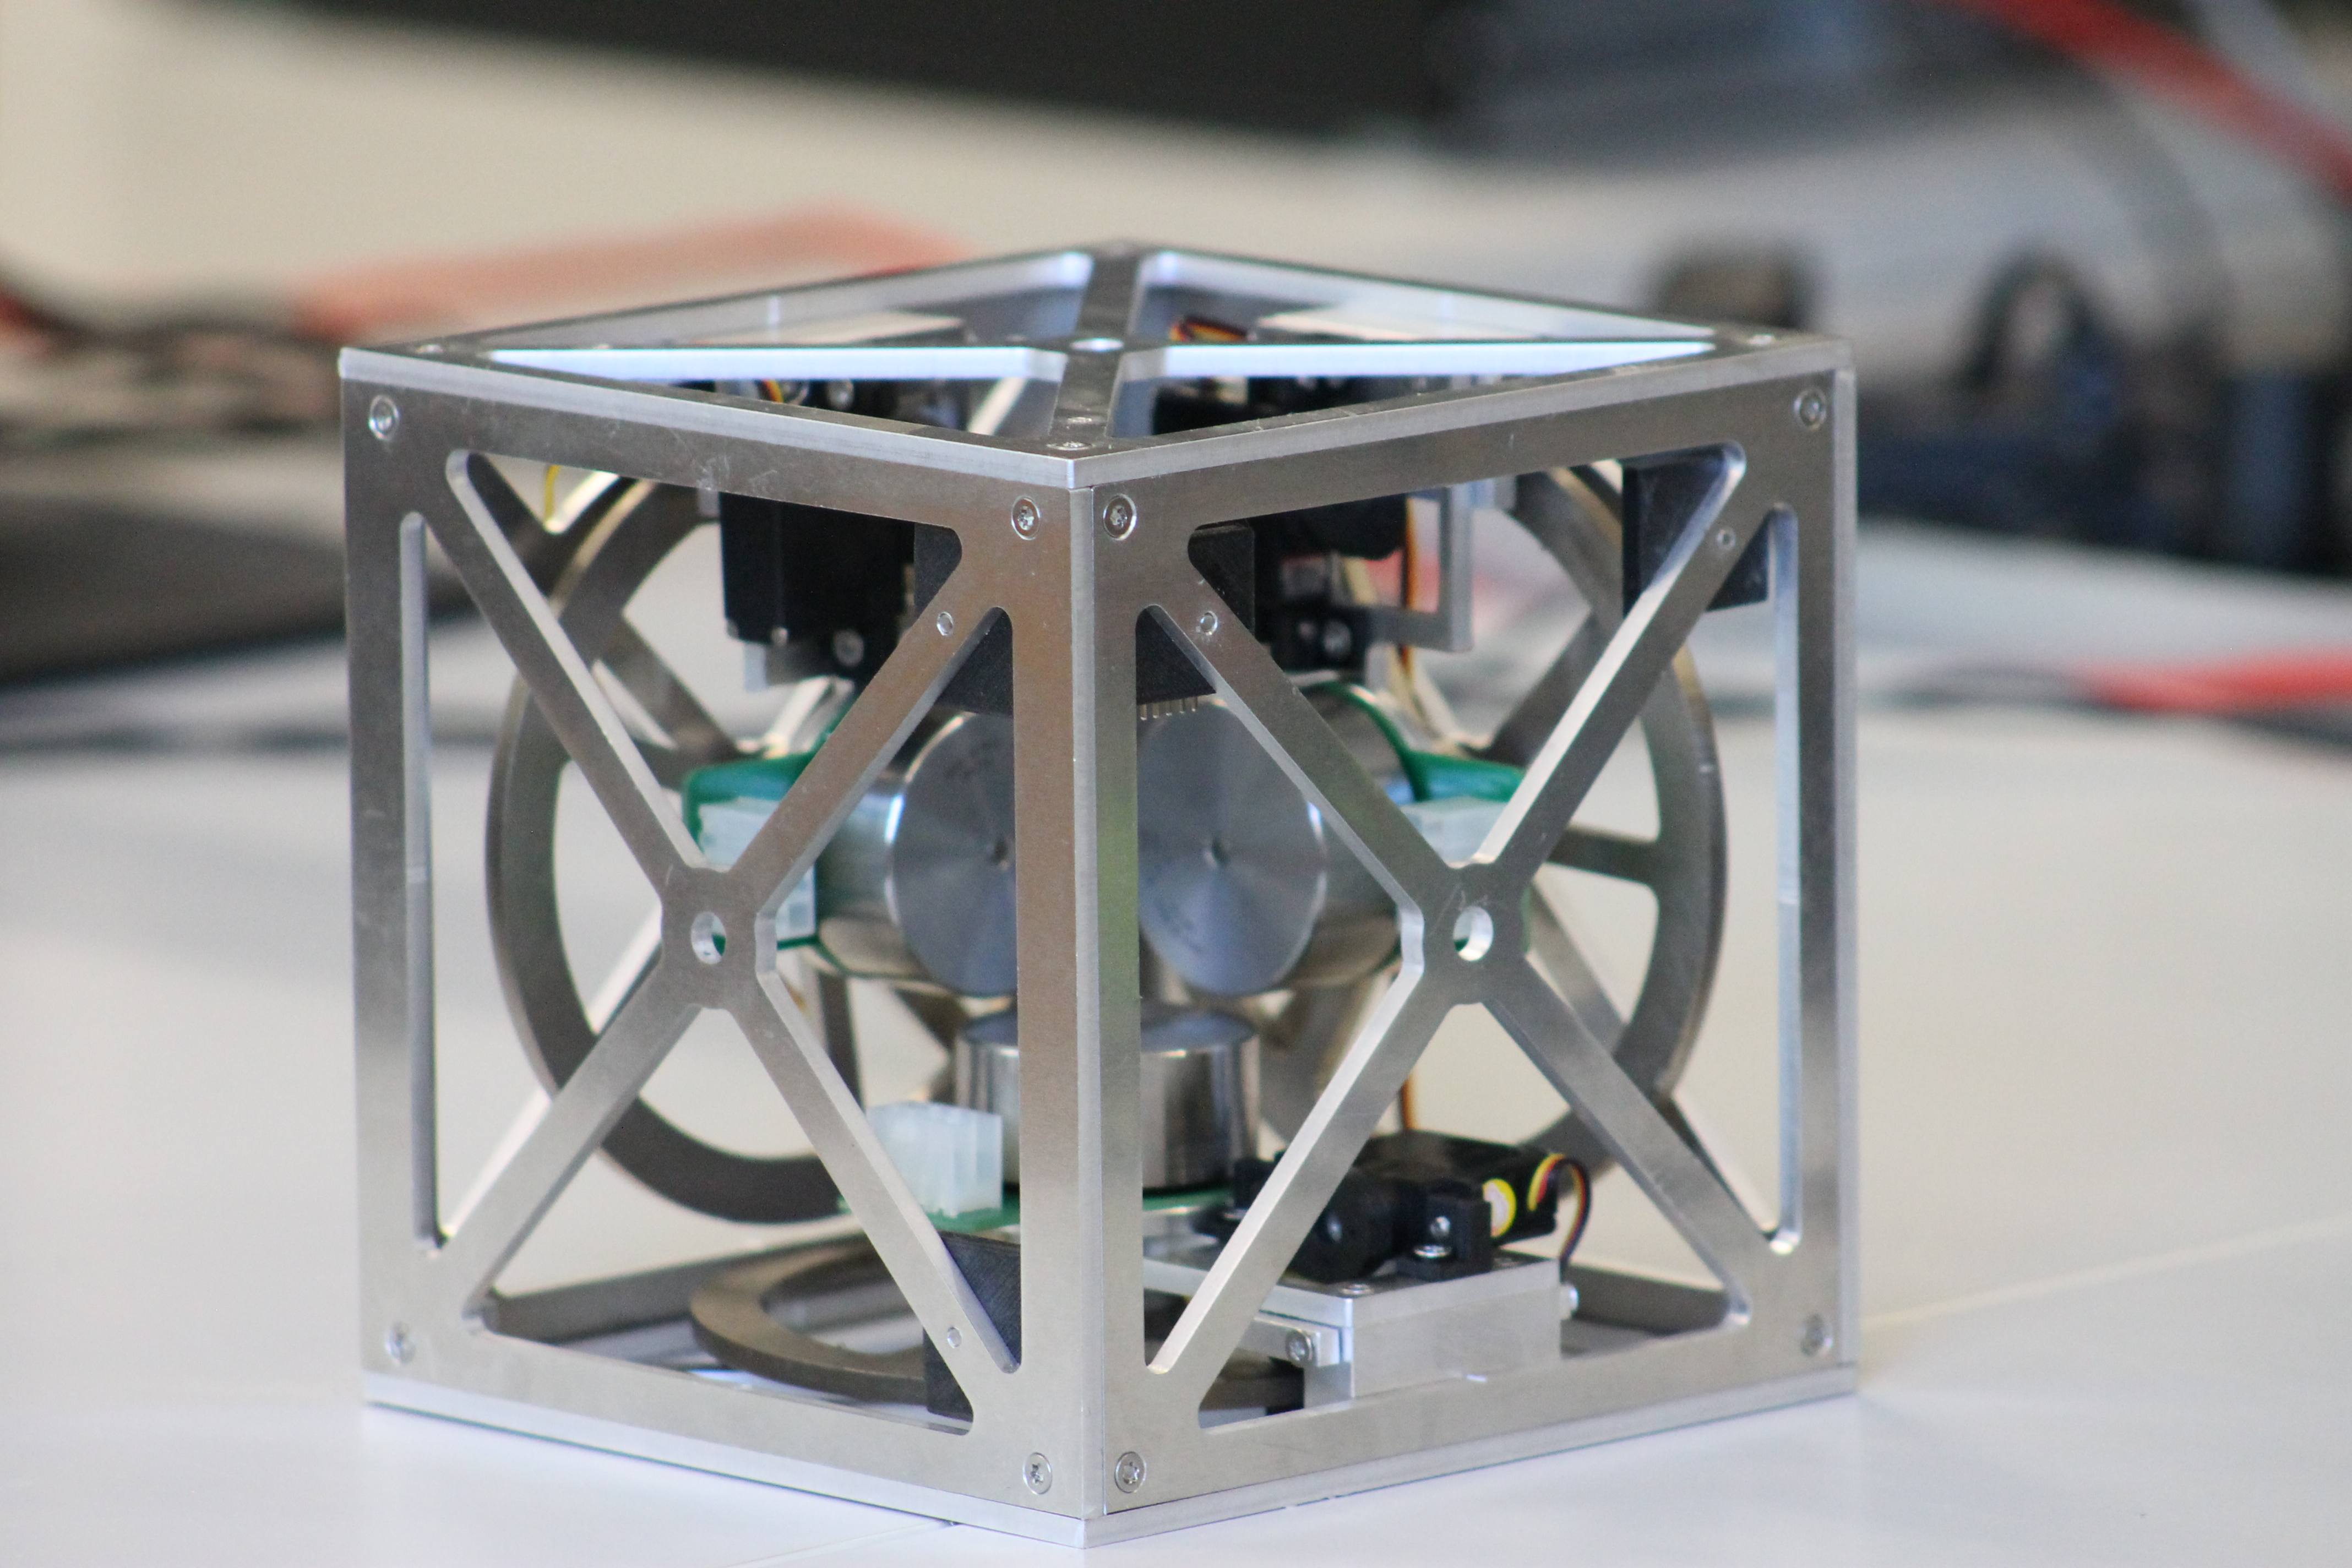
\includegraphics[width=\linewidth]{img/3D_Modell_img.JPG}
\caption{3D-Modell, Quelle: eigene Darstellung}
\end{figure}